\documentclass[noinstructornotes]{ximera}
%% handout
%% space
%% newpage
%% numbers
%% nooutcomes

%I added the commands here so that I would't have to keep looking them up
%\newcommand{\RR}{\mathbb R}
%\renewcommand{\d}{\,d}
%\newcommand{\dd}[2][]{\frac{d #1}{d #2}}
%\renewcommand{\l}{\ell}
%\newcommand{\ddx}{\frac{d}{dx}}
%\everymath{\displaystyle}
%\newcommand{\dfn}{\textbf}
%\newcommand{\eval}[1]{\bigg[ #1 \bigg]}

%\begin{image}
%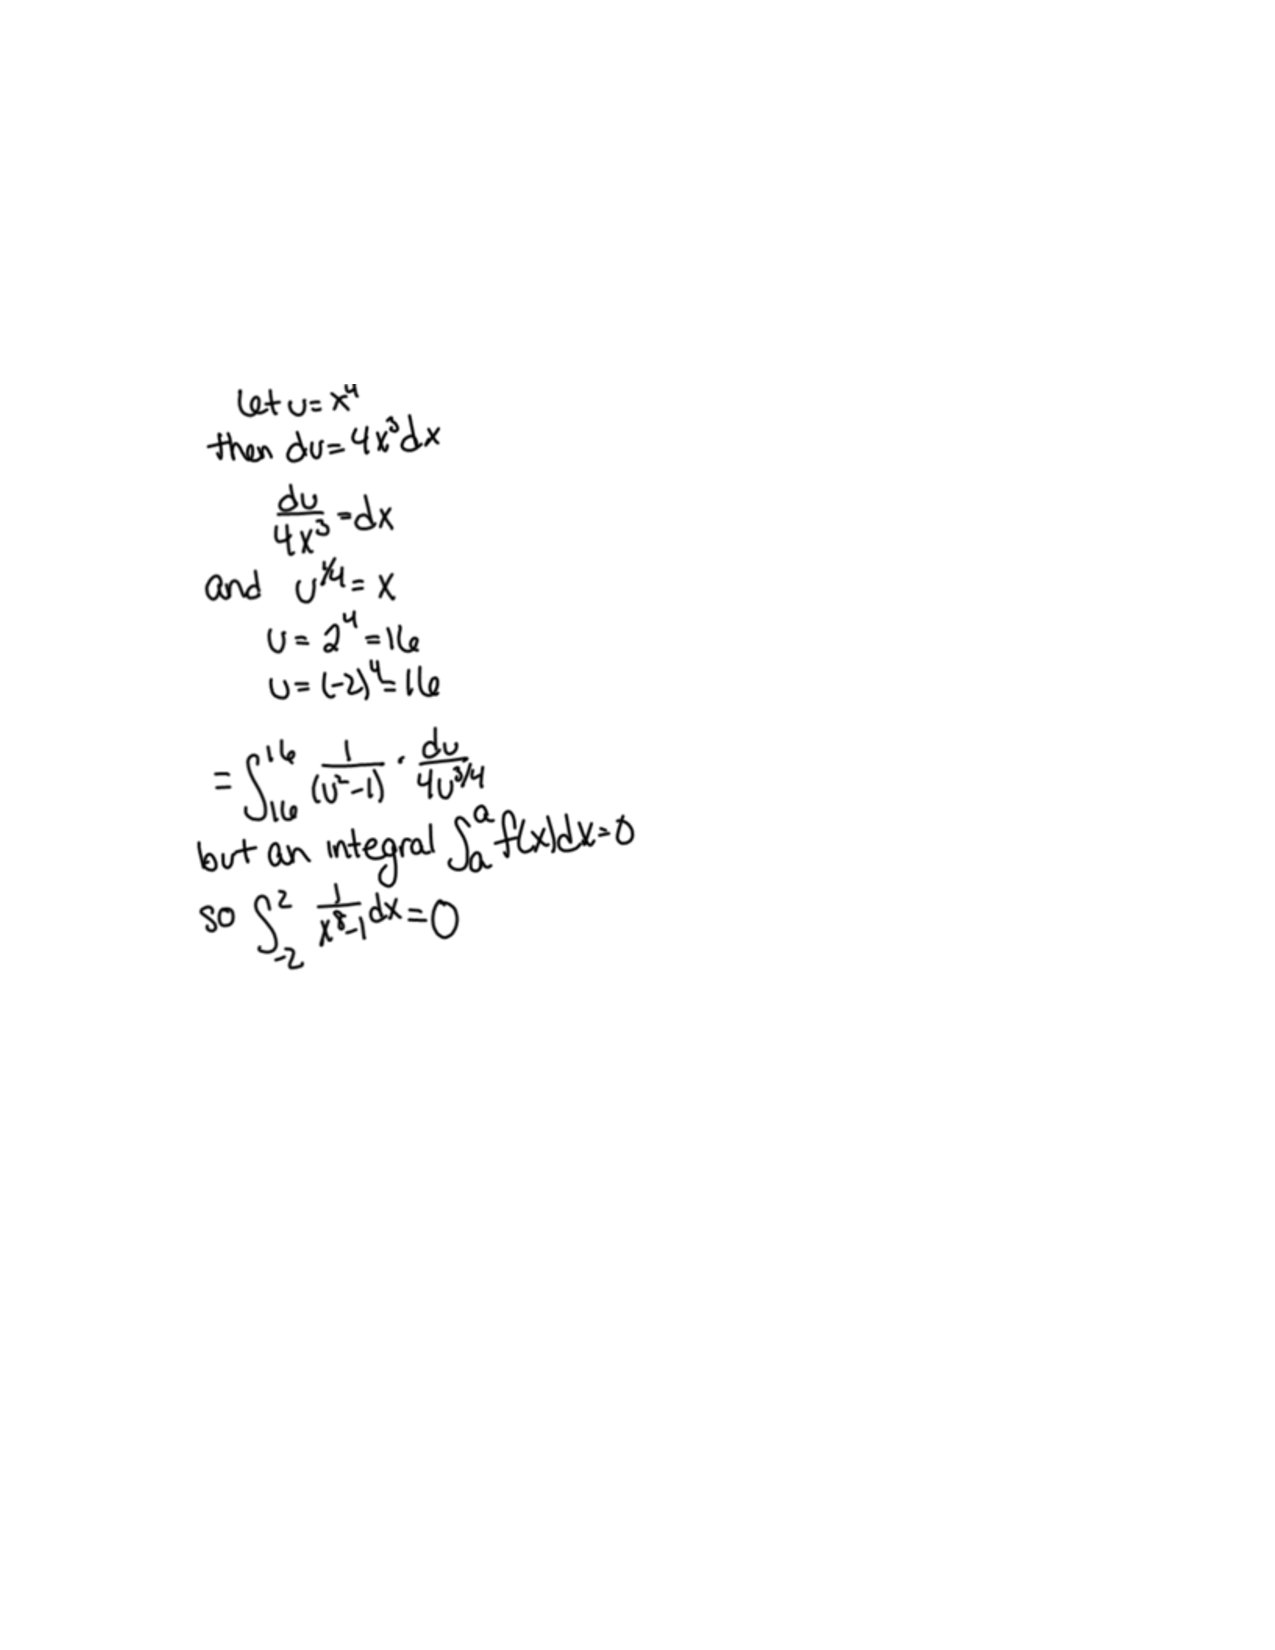
\includegraphics[trim= 170 420 250 180]{Figure1.pdf}
%\end{image}


\newcommand{\RR}{\mathbb R}
\renewcommand{\d}{\,d}
\newcommand{\dd}[2][]{\frac{d #1}{d #2}}
\renewcommand{\l}{\ell}
\newcommand{\ddx}{\frac{d}{dx}}
\newcommand{\dfn}{\textbf}
\newcommand{\eval}[1]{\bigg[ #1 \bigg]}

\usepackage{multicol}

\renewenvironment{freeResponse}{
\ifhandout\setbox0\vbox\bgroup\else
\begin{trivlist}\item[\hskip \labelsep\bfseries Solution:\hspace{2ex}]
\fi}
{\ifhandout\egroup\else
\end{trivlist}
\fi} %% we can turn off input when making a master document

\title{Recitation \#1 - Review of Integration}  

\begin{document}
\begin{abstract}		\end{abstract}
\maketitle



The following worksheet is designed to help review and/or sharpen your ability to differentiate and integrate functions encountered in a typical Calculus 1 course.  


\section{Group work:}



%problem 1
\begin{problem}
Consider the function $f(x)=e^{2x}$.  We know that $\dfrac{d}{dx} \left( e^{2x} \right) = 2 e^{2x}$ by the Chain Rule, and this lets us easily conclude that $\int e^{2x} \, dx = \frac{1}{2} e^{2x}$.  This could of course be verified by u-substitution (if you know/remember this technique), but can also be understood the following way:

The symbol $\int e^{2x} \, dx$ represents a function whose derivative is $e^{2x}$.  Since taking a derivative of $e^{2x}$ results in multiplying $e^{2x}$ by 2, when we antidifferentiate $e^{2x}$, we must multiply by $\frac{1}{2}$.  

You must be careful with this type of thought!  Indeed, it works only when the argument of the function (in this case, the expression in the exponent) is LINEAR.  ``Linear in x" means the argument is of the form $ax+b$ in x!

	\begin{enumerate}
	
	%part a
	\item  Calculate $\dfrac{d}{dx} \left(e^{x^2} \right) $.
	\begin{freeResponse}
		$\dfrac{d}{dx} \left(e^{x^2} \right) = e^{x^2} \left( 2^x \right)' = e^{x^2} \left( 2x \right)$
	\end{freeResponse}
			
		
	%part b
	\item Suppose a student tries to apply the above logic to compute $\int e^{x^2} \, dx$.  The student concludes that since $\dfrac{d}{dx} e^{x^2} \, dx = 2x e^{x^2} $, then: 
\begin{equation}
 \int e^{x^2} \, dx = \dfrac{1}{2x} e^{x^2} \label{bad1}
\end{equation}

Since you know that $\int e^{x^2} \, dx$ is a function whose derivative is $e^{x^2}$, prove this student wrong by differentiating his/her answer (i.e. the RHS of Eqn \ref{bad1}).  
	\begin{freeResponse}
	First, the student forgot "+C" ! \\
	Also, if the student is correct, then the derivative of his/her answer should be $e^{x^2}$, but:\\
	$\dfrac{d}{dx} \left( \frac{1}{2x} e^{x^2} \right) = \frac{\left(e^{x^2}\right)' \cdot 2x - e^{x^2} \left( 2x \right)'}{\left( 2x \right)^2} = 
	\frac{4x^2e^{x^2} - 2e^{x^2}}{4x^2}$ \\
	This is not $e^{x^2}$!
	\end{freeResponse}
		
	%part c
	\item 	What insight does this reveal as to why this students' answer is wrong?  Why can we think of antidifferentiating $e^{2x}$ differently than antidifferentiating $e^{x^2}$?
		
			\begin{freeResponse}
			Note that to differentiate $ \frac{1}{2x} e^{x^2} $, we need the quotient rule!  When we differentiate $ \frac{1}{2} e^{x^2}$, we don't need the quotient rule because $\frac{1}{2}$ is just a constant. \\
			Whenever the arguement is linear in x, the derivative of the argument will be a constant, so we won't need the quotient rule.  Indeed, if $F'(x) = f(x)$, then $\int f(ax+b) \, dx = \frac{1}{a}F(ax+b) + C$ since \\ 
			$\dfrac{d}{dx} \left( \frac{1}{a} F(ax+b) \right) = \frac{1}{a} F'(ax+b) \cdot (ax+b)' = \frac{1}{a}f(ax+b) \cdot a = f(ax+b)$
			\end{freeResponse}
	\end{enumerate}
		
		
\end{problem}

%problem 2
\begin{problem}
Categorize the following integrals into ones you know how to integrate after taking Calculus 1 and learning section 7.1 and ones you do not know how to integrate.  If you have time, try to evaluate the integrals.

\begin{align*}
a) & \int \left(3x^4-\sqrt[3]{x^2} + \dfrac{2}{\sqrt[7]{x}}\right)  \, dx  & b) & \int e^{x^2} \, dx & c) & \int^{\pi/6}_{0} 4 \sin(2x) \, dx  \\
d) & \int e^{-\frac{x}{3}} \, dx  & e) & \int \ln x \, dx & f) & \int \dfrac{4x^3-3x}{2x^2} \, dx  \\
g) & \int \left( \sec(4x) \tan(4x) + 3 \sec^2 \frac{x}{5} \right) \, dx  & h) & \int^4_1 (\sqrt{x}-1)^2 \, dx  & i) & \int_0^1 \sqrt{e^{3x}} \, dx  \\
j) &\int \cot^2 (3x) \sec^2 (3x) \, dx & k) & \int \cos \sqrt{x} \, dx & l) & \int \dfrac{2}{(3x)^2} \\
\end{align*}
			
	\begin{freeResponse}		
	See attached solutions section II
	\end{freeResponse}
		
\end{problem}

On your own:
%problem 3
\begin{problem}

Differentiate the following functions.
\begin{align*}
a)  \, \, y &= (2x-7)^4  & b) \, \, y &=  e^{\frac{x}{4}} & c) \, \, y&= 7x^4-3\sqrt[5]{x} + \dfrac{2}{5x^2} \\
d) \, \, y&= \ln(2x+\cos x) & e) \, \, y&=2xe^{-x} & f) \, \, y&= \dfrac{\tan{(3x)}}{\sqrt{4-x}} \\
g) \, \, y&= \csc{\left(e^{4x}\right)} & h) \, \, y&= [\ln(4x^3-2x)]^3 & i) \, \, y&= e^{4 \sqrt{x}} \\
j) \, \, y&=4e^{x \sin x} & k) \, \, y&= 6x^9-\dfrac{1}{8x^4}+\dfrac{2}{\sqrt[3]{2x-1}} & l) \, \, y &=\dfrac{2}{(3x^2-1)^2} \\
\end{align*}

	\begin{freeResponse}		
	See attached solutions section I
	\end{freeResponse}


	
\end{problem}


\end{document} 


















